\documentclass[t,aspectratio=169]{beamer}
%\usetheme{Berkeley}
\usepackage{graphicx}
\usepackage{amsmath}
\usepackage[american]{circuitikz}

\title{Clase 15}
\subtitle{Polarización BJT}
\author{Dr.-Ing. Juan José Montero Rodríguez}
\subject{Elementos Activos}
\institute{Escuela de Ingeniería Electrónica}
\date{Semestre II-2023}

\begin{document}

\begin{frame}{}
\maketitle
\end{frame}

\section{Polarización fija}
\begin{frame}{Polarización por resistencia de base}

El circuito de \textbf{polarización fija} se muestra a continuación:

\begin{figure}
    \centering
    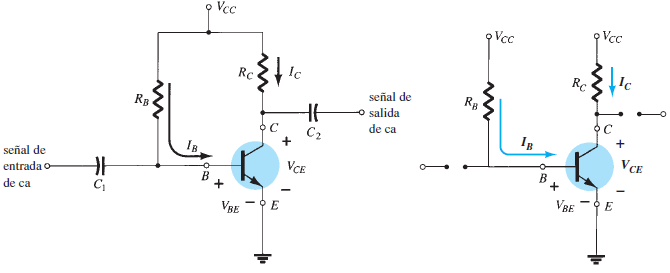
\includegraphics[width=0.8\textwidth]{figures/polarizacion_fija.png}
\end{figure}

Los \textbf{condensadores de desacople} se consideran circuitos abiertos en CD, y cortocircuitos en CA (la reactancia es $X_C = 1/j\omega{}C$ y es muy baja si $C$ es alto).

\end{frame}


\begin{frame}{Análisis del circuito de polarización fija}

\begin{columns}
\begin{column}{0.25\textwidth}

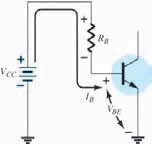
\includegraphics[width=\textwidth]{figures/polarizacion_fija_analisis.png}

\end{column}
\begin{column}{0.75\textwidth}

Primero necesitamos obtener la ecuación del circuito.

La malla por la base:
%
\[ V_{CC} = I_B R_B + V_{BE} \]
%
\[ V_{CC} = \dfrac{I_C}{\beta} R_B + V_{BE} \]
%
\[ I_C = \beta \left( \dfrac{V_{CC} - V_{BE}}{R_B} \right) \]

La segunda ecuación depende del modelo del transistor.

\begin{itemize}
    \item Con el modelo de tensión constante, $V_{BE} = 0.7\ V$.
    \item Con el modelo exponencial, $V_{BE} = V_t \ln I_C/I_S$.
\end{itemize}

La solución de este sistema de dos ecuaciones da como resultado el punto de operación.

\end{column}
\end{columns}
    
\end{frame}


\begin{frame}{Ejemplo 1: Polarización fija}

Para el circuito de la figura, determine $I_B$, $I_C$, $V_{CE}$, $V_B$, $V_C$, $V_{BC}$. 

Utilice el modelo de tensión constante con $V_{BE} = 0.7\ V$.

\begin{figure}
    \centering
    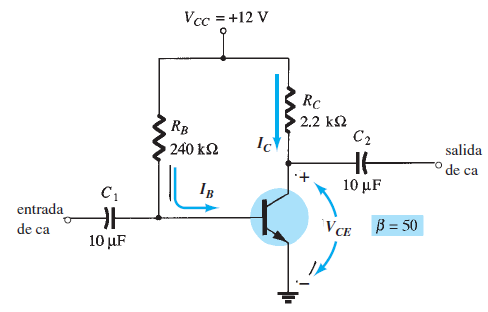
\includegraphics[width=0.6\textwidth]{figures/polarizacion_fija_ejemplo.png} 
\end{figure}

\end{frame}


\begin{frame}{Solución 1: Polarización fija}

\begin{figure}
    \flushleft
    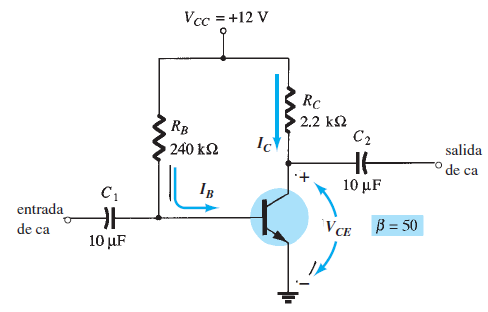
\includegraphics[width=0.5\textwidth]{figures/polarizacion_fija_ejemplo.png} 
\end{figure}

\end{frame}

\begin{frame}{Solución 1: Polarización fija}

\begin{figure}
    \flushleft
    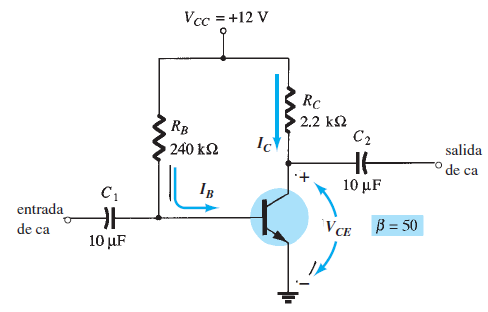
\includegraphics[width=0.5\textwidth]{figures/polarizacion_fija_ejemplo.png} 
\end{figure}

\end{frame}


\section{Polarización fija con RE}
\begin{frame}{Polarización fija con resistencia de emisor}

La resistencia de emisor mejora la estabilidad del circuito:

\begin{figure}
    \centering
    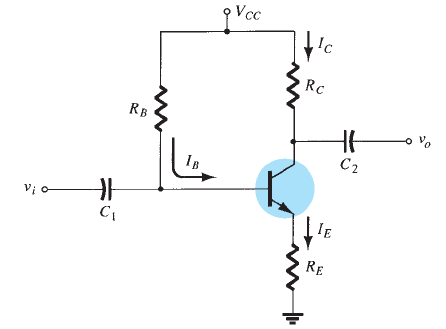
\includegraphics[width=0.5\textwidth]{figures/polarizacion_fija_RE.png}
\end{figure}

Esta configuración es más estable ante variaciones de $\beta$, tolerancia en la resistencia $R_B$ y variaciones de temperatura.

\end{frame}


\begin{frame}{Análisis del circuito de polarización fija con RE}

\begin{columns}
\begin{column}{0.5\textwidth}

\begin{figure}
    \centering
    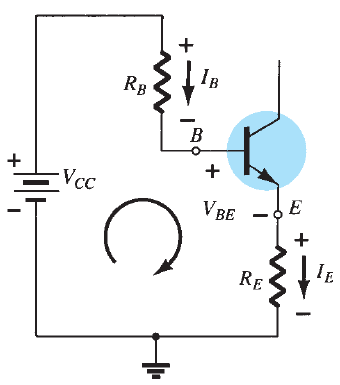
\includegraphics[width=0.6\textwidth]{figures/polarizacion_fija_RE_analisis.png}
\end{figure}

\end{column}
\begin{column}{0.5\textwidth}

La malla por la base:
%
\[ V_{CC} = I_B R_B + V_{BE} + I_E R_E \]
%
\[ V_{CC} = \dfrac{I_C}{\beta} R_B + V_{BE} + \dfrac{\beta + 1}{\beta} I_C R_E \]
%
\[ V_{CC} - V_{BE} = I_C \left( \dfrac{R_B}{\beta}  + \dfrac{\beta + 1}{\beta} R_E \right)  \]
%
\[ I_C = \dfrac{V_{CC} - V_{BE}}{ \dfrac{R_B}{\beta}  + \dfrac{\beta + 1}{\beta} R_E }  \]

Esta ecuación se resuelve junto con la ecuación del modelo del transistor para obtener el punto de operación.

\end{column}
\end{columns}

\end{frame}


\begin{frame}{Ejemplo 2: Polarización fija con RE}

\begin{figure}
    \centering
    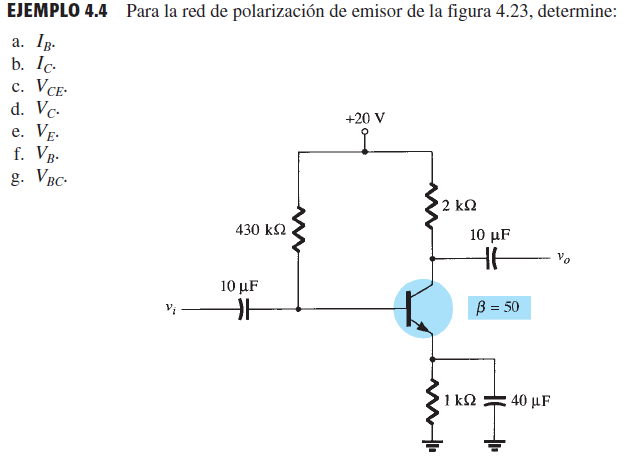
\includegraphics[width=0.7\textwidth]{figures/polarizacion_fija_RE_ejemplo.png}
\end{figure}
    
\end{frame}



\begin{frame}{Solución 2: Polarización fija con RE}

\begin{figure}
    \flushleft
    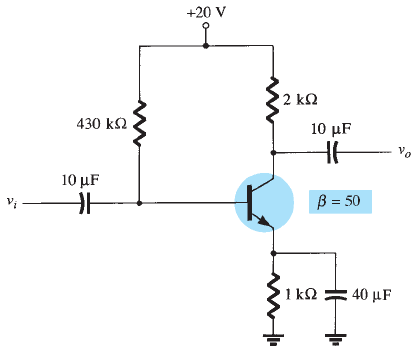
\includegraphics[width=0.4\textwidth]{figures/polarizacion_fija_RE_solucion.png}
\end{figure}

\end{frame}



\begin{frame}{Solución 2: Polarización fija con RE}

\begin{figure}
    \flushleft
    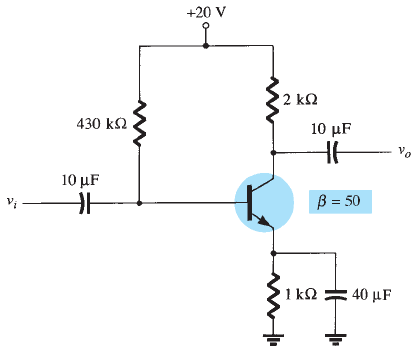
\includegraphics[width=0.4\textwidth]{figures/polarizacion_fija_RE_solucion.png}
\end{figure}
    
\end{frame}




\section{Polarización por divisor de tensión}
\begin{frame}{Polarización por divisor de tensión}

La tensión de la base se puede establecer por un divisor de tensión:

\begin{figure}
    \centering
    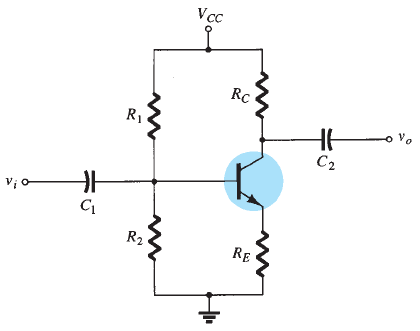
\includegraphics[width=0.5\textwidth]{figures/polarizacion_divisor_tension.png}
\end{figure}

En este circuito, la polarización es independiente de $\beta$.


\end{frame}


\begin{frame}{Análisis de la polarización por divisor de tensión (solución aproximada)}

\begin{columns}
\begin{column}{0.5\textwidth}

\begin{figure}
    \centering
    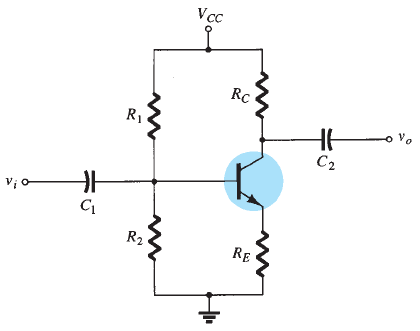
\includegraphics[width=\textwidth]{figures/polarizacion_divisor_tension.png}
\end{figure}

\end{column}
\begin{column}{0.5\textwidth}

\textbf{Solución aproximada}

Suponiendo que la corriente de base es despreciable:
%
\[ V_B = \dfrac{V_{CC} \times R_2}{R_1  + R_2 }  \]
%
\[ V_E = I_E R_E \]
%
\[ V_{BE} = V_B - V_E \]
%
\[ I_C = I_S \left( e^{V_{BE}/V_t} - 1 \right) \]
%
\[ I_C = I_S \cdot e^{\left(\dfrac{V_{CC} \times R_2}{R_1  + R_2 }-I_E R_E\right)/V_t} \]

\end{column}
\end{columns}

\end{frame}


\begin{frame}{Análisis de la polarización por divisor de tensión (solución exacta)}

\begin{columns}
\begin{column}{0.5\textwidth}

\begin{figure}
    \centering
    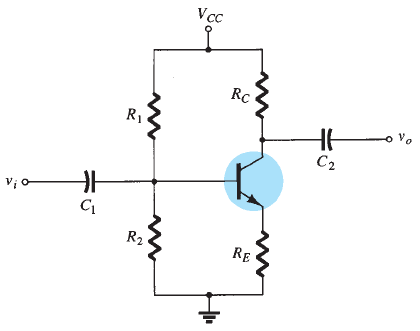
\includegraphics[width=\textwidth]{figures/polarizacion_divisor_tension.png}
\end{figure}

\end{column}
\begin{column}{0.5\textwidth}

\textbf{Solución exacta}

Se resuelve por equivalente de Thévenin:

\begin{figure}
    \centering
    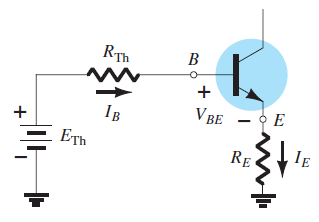
\includegraphics[width=5cm]{figures/polarizacion_divisor_thevenin.png}
\end{figure}
%
\[ V_{THV} = \dfrac{V_{CC} \times R_2}{R_1 + R_2} \]

\[ R_{THV} = R_1 \parallel R_2 \]

\end{column}
\end{columns}

\end{frame}


\begin{frame}{Ejemplo 3: Polarización por divisor de tensión}

\begin{columns}
\begin{column}{0.5\textwidth}

\begin{figure}
    \centering
    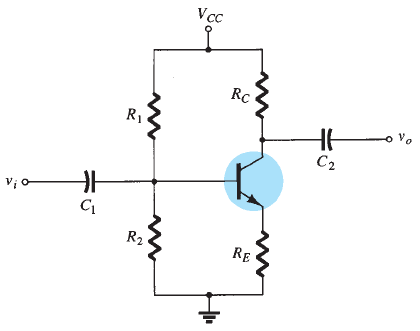
\includegraphics[width=\textwidth]{figures/polarizacion_divisor_tension.png}
\end{figure}

\end{column}
\begin{column}{0.5\textwidth}

Determine la corriente del circuito, suponiendo los siguientes valores:

\[ V_{CC} = 3\ V \]
%
\[ R_1 = 11\ k\Omega \]
%
\[ R_2 = 14\ k\Omega \]
%
\[ R_E = 47\ \Omega \]
%
\[ R_C = 100\ \Omega \]
%
\[ I_S = 3\times{}10^{-14}\ A \]
%
\[ \beta = 100 \]

\end{column}
\end{columns}

\end{frame}


\begin{frame}{Solución 3: Polarización por divisor de tensión}

\begin{columns}
\begin{column}{0.5\textwidth}

\begin{figure}
    \centering
    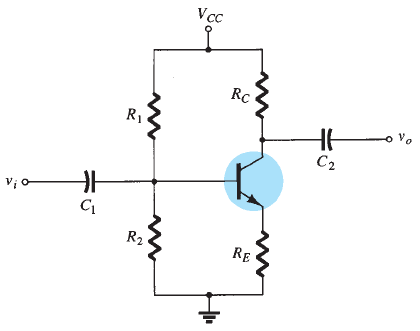
\includegraphics[width=\textwidth]{figures/polarizacion_divisor_tension.png}
\end{figure}

\end{column}
\begin{column}{0.5\textwidth}


\end{column}
\end{columns}

\end{frame}



\begin{frame}{Solución 3: Polarización por divisor de tensión}

\begin{columns}
\begin{column}{0.5\textwidth}

\begin{figure}
    \centering
    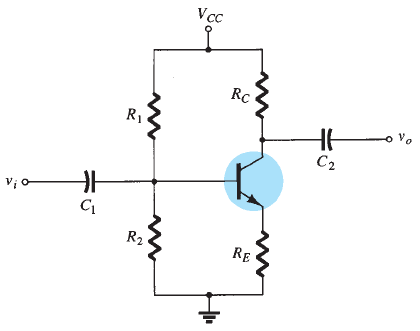
\includegraphics[width=\textwidth]{figures/polarizacion_divisor_tension.png}
\end{figure}

\end{column}
\begin{column}{0.5\textwidth}


\end{column}
\end{columns}

\end{frame}


\section{Autopolarización}
\begin{frame}{Autopolarización}

El circuito de autopolarización utiliza la tensión de colector para polarizar la base.

\begin{columns}
\begin{column}{0.5\textwidth}

\begin{figure}[H]
    \centering
    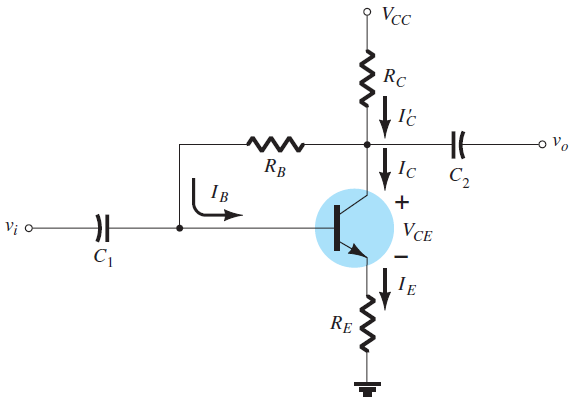
\includegraphics[width=\textwidth]{figures/polarizacion_autopolarizacion.png}
\end{figure}

\end{column}
\begin{column}{0.5\textwidth}

\begin{figure}[H]
    \centering
    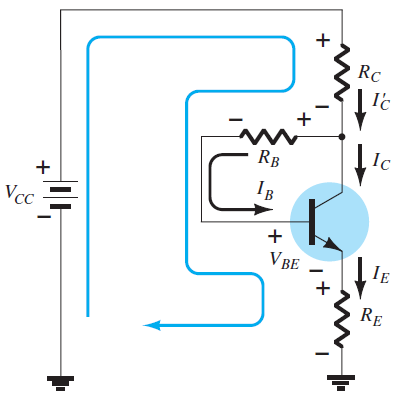
\includegraphics[width=0.7\textwidth]{figures/polarizacion_autopolarizacion_2.png}
\end{figure}

\end{column}
\end{columns}

\end{frame}


\begin{frame}{Análisis del circuito de autopolarización}


\begin{columns}
\begin{column}{0.35\textwidth}

\begin{figure}[H]
    \centering
    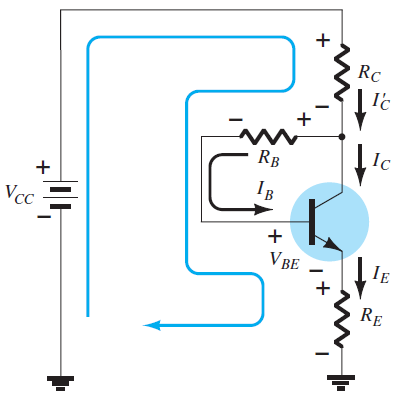
\includegraphics[width=\textwidth]{figures/polarizacion_autopolarizacion_2.png}
\end{figure}

\end{column}
\begin{column}{0.65\textwidth}

Se analiza la malla por la base:
%
\[ V_{CC} - I_C'R_C - I_B R_B - V_{BE} - I_E R_E = 0 \]
%
\[ V_{CC} - (I_C + I_B) R_C - I_B R_B - V_{BE} - I_E R_E = 0 \]
%
\[ V_{CC} - (\beta I_B + I_B) R_C - I_B R_B - V_{BE} - (\beta + 1) I_B R_E = 0 \]
%
\[ I_B = \dfrac{V_{CC} - V_{BE}}{(\beta + 1) R_C + R_B + (\beta + 1) R_E} \]
%
\[ I_C = \dfrac{\beta(V_{CC} - V_{BE})}{(\beta + 1) R_C + R_B + (\beta + 1) R_E} \]

Esta ecuación se resuelve junto con la ecuación del modelo del transistor.
\end{column}
\end{columns}

\end{frame}


\section{Referencias}

\begin{frame}{Lecturas recomendadas}

\begin{itemize}
    \item Boylestad, R. y Nashelsky, L. (2009). Electrónica: Teoría de circuitos y dispositivos electrónicos. Capítulo 4: Polarización de cd de los BJT, pp. 161-200, Pearson Educación, México.
\end{itemize}

\end{frame}

\end{document}
